\documentclass[a4paper,
fontsize=11pt,
%headings=small,
oneside,
numbers=noperiodatend,
parskip=half-,
bibliography=totoc,
final
]{scrartcl}

\usepackage[babel]{csquotes}
\usepackage{synttree}
\usepackage{graphicx}
\setkeys{Gin}{width=.8\textwidth} %default pics size

\graphicspath{{./plots/}}
\usepackage[ngerman]{babel}
\usepackage[T1]{fontenc}
%\usepackage{amsmath}
\usepackage[utf8x]{inputenc}
\usepackage [hyphens]{url}
\usepackage{booktabs} 
\usepackage[left=2.4cm,right=2.4cm,top=2.3cm,bottom=2cm,includeheadfoot]{geometry}
\usepackage[labelformat=empty]{caption} % option 'labelformat=empty]' to surpress adding "Abbildung 1:" or "Figure 1" before each caption / use parameter '\captionsetup{labelformat=empty}' instead to change this for just one caption
\usepackage{eurosym}
\usepackage{multirow}
\usepackage[ngerman]{varioref}
\setcapindent{1em}
\renewcommand{\labelitemi}{--}
\usepackage{paralist}
\usepackage{pdfpages}
\usepackage{lscape}
\usepackage{float}
\usepackage{acronym}
\usepackage{eurosym}
\usepackage{longtable,lscape}
\usepackage{mathpazo}
\usepackage[normalem]{ulem} %emphasize weiterhin kursiv
\usepackage[flushmargin,ragged]{footmisc} % left align footnote
\usepackage{ccicons} 
\setcapindent{0pt} % no indentation in captions
\usepackage{xurl} % Breaks URLs

%%%% fancy LIBREAS URL color 
\usepackage{xcolor}
\definecolor{libreas}{RGB}{112,0,0}

\usepackage{listings}

\urlstyle{same}  % don't use monospace font for urls

\usepackage[fleqn]{amsmath}

%adjust fontsize for part

\usepackage{sectsty}
\partfont{\large}

%Das BibTeX-Zeichen mit \BibTeX setzen:
\def\symbol#1{\char #1\relax}
\def\bsl{{\tt\symbol{'134}}}
\def\BibTeX{{\rm B\kern-.05em{\sc i\kern-.025em b}\kern-.08em
    T\kern-.1667em\lower.7ex\hbox{E}\kern-.125emX}}

\usepackage{fancyhdr}
\fancyhf{}
\pagestyle{fancyplain}
\fancyhead[R]{\thepage}

% make sure bookmarks are created eventough sections are not numbered!
% uncommend if sections are numbered (bookmarks created by default)
\makeatletter
\renewcommand\@seccntformat[1]{}
\makeatother

% typo setup
\clubpenalty = 10000
\widowpenalty = 10000
\displaywidowpenalty = 10000

\usepackage{hyperxmp}
\usepackage[colorlinks, linkcolor=black,citecolor=black, urlcolor=libreas,
breaklinks= true,bookmarks=true,bookmarksopen=true]{hyperref}
\usepackage{breakurl}

%meta

%meta

\fancyhead[L]{B. Kaden\\ %author
LIBREAS. Library Ideas, 46 (2024). % journal, issue, volume.
\href{https://doi.org/10.18452/31227}{\color{black}https://doi.org/10.18452/31227}
{}} % doi 
\fancyhead[R]{\thepage} %page number
\fancyfoot[L] {\ccLogo \ccAttribution\ \href{https://creativecommons.org/licenses/by/4.0/}{\color{black}Creative Commons BY 4.0}}  %licence
\fancyfoot[R] {ISSN: 1860-7950}

\title{\LARGE{Kolumne Bibliotheksphilokartie: Eine Erinnerungskarte aus Berlin-Friedrichshain}}% title
\author{Ben Kaden} % author

\setcounter{page}{1}

\hypersetup{%
      pdftitle={Kolumne Bibliotheksphilokartie: Eine Erinnerungskarte aus Berlin-Friedrichshain},
      pdfauthor={Ben Kaden},
      pdfcopyright={CC BY 4.0 International},
      pdfsubject={LIBREAS. Library Ideas, 46 (2024)},
      pdfkeywords={DDR, Postkarte, Bibliothek, Erinnerung},
      pdflicenseurl={https://creativecommons.org/licenses/by/4.0/},
      pdfcontacturl={http://libreas.eu},
      baseurl={},
      pdflang={de},
      pdfmetalang={de},
      pdfdoi={10.18452/31227},
      pdfurl={https://doi.org/10.18452/31227}
     }



\date{}
\begin{document}

\maketitle
\thispagestyle{fancyplain} 

%abstracts

%body
Im Jahr 1984 gab es in Berlin-Friedrichshain ein Dutzend öffentliche
Bibliotheken. So lautet jedenfalls die gedruckte Auskunft des
Telefonbuchs für Ost-Berlin aus diesem Jahr. Neben der zentral
zuständigen Pablo-Neruda-Bibliothek in der Mollstraße / Ecke
Hans-Beimler-Straße, die sogar eine Linguathek mit zum Beispiel
arabischen oder japanischen Selbstlernkursen vorhielt\footnote{Neues
  Deutschland, 14.08.1984, S.\,8}, waren es sechs
\enquote{Erwachsenenbibliotheken} und fünf Kinderbibliotheken zur
Versorgung der um die 120.000 Einwohner des Stadtbezirks. Eine dieser
Bibliotheken befand sich in der Wedekindstraße 24 und zwar ziemlich
direkt gegenüber des Hauses, das 20 Jahre später Drehort für die Wohnung
Georg Dreymans, der observierten Hauptfigur in Florian Henckel von
Donnersmarcks \enquote{Das Leben der Anderen} werden sollte. Um die Ecke
und Stück weiter die Gubener Straße Richtung Comeniusplatz und dann noch
ein paar Meter weiter wohnte ein Tony. Und pünktlich zum
Schuljahresbeginn, nämlich mit Poststempel vom 30. August 1984,
versuchte ein Briefträger oder eine Briefträgerin eine
Erinnerungspostkarte zuzustellen, die diesen Sommer, also vierzig Jahre
später zufällig in meine Sammlung geriet. Wo sie die Zwischenzeit
verbrachte, lässt sich, wie bei Flohmarktentdeckungen üblich, nicht
rekonstruieren.

\begin{figure}
\centering
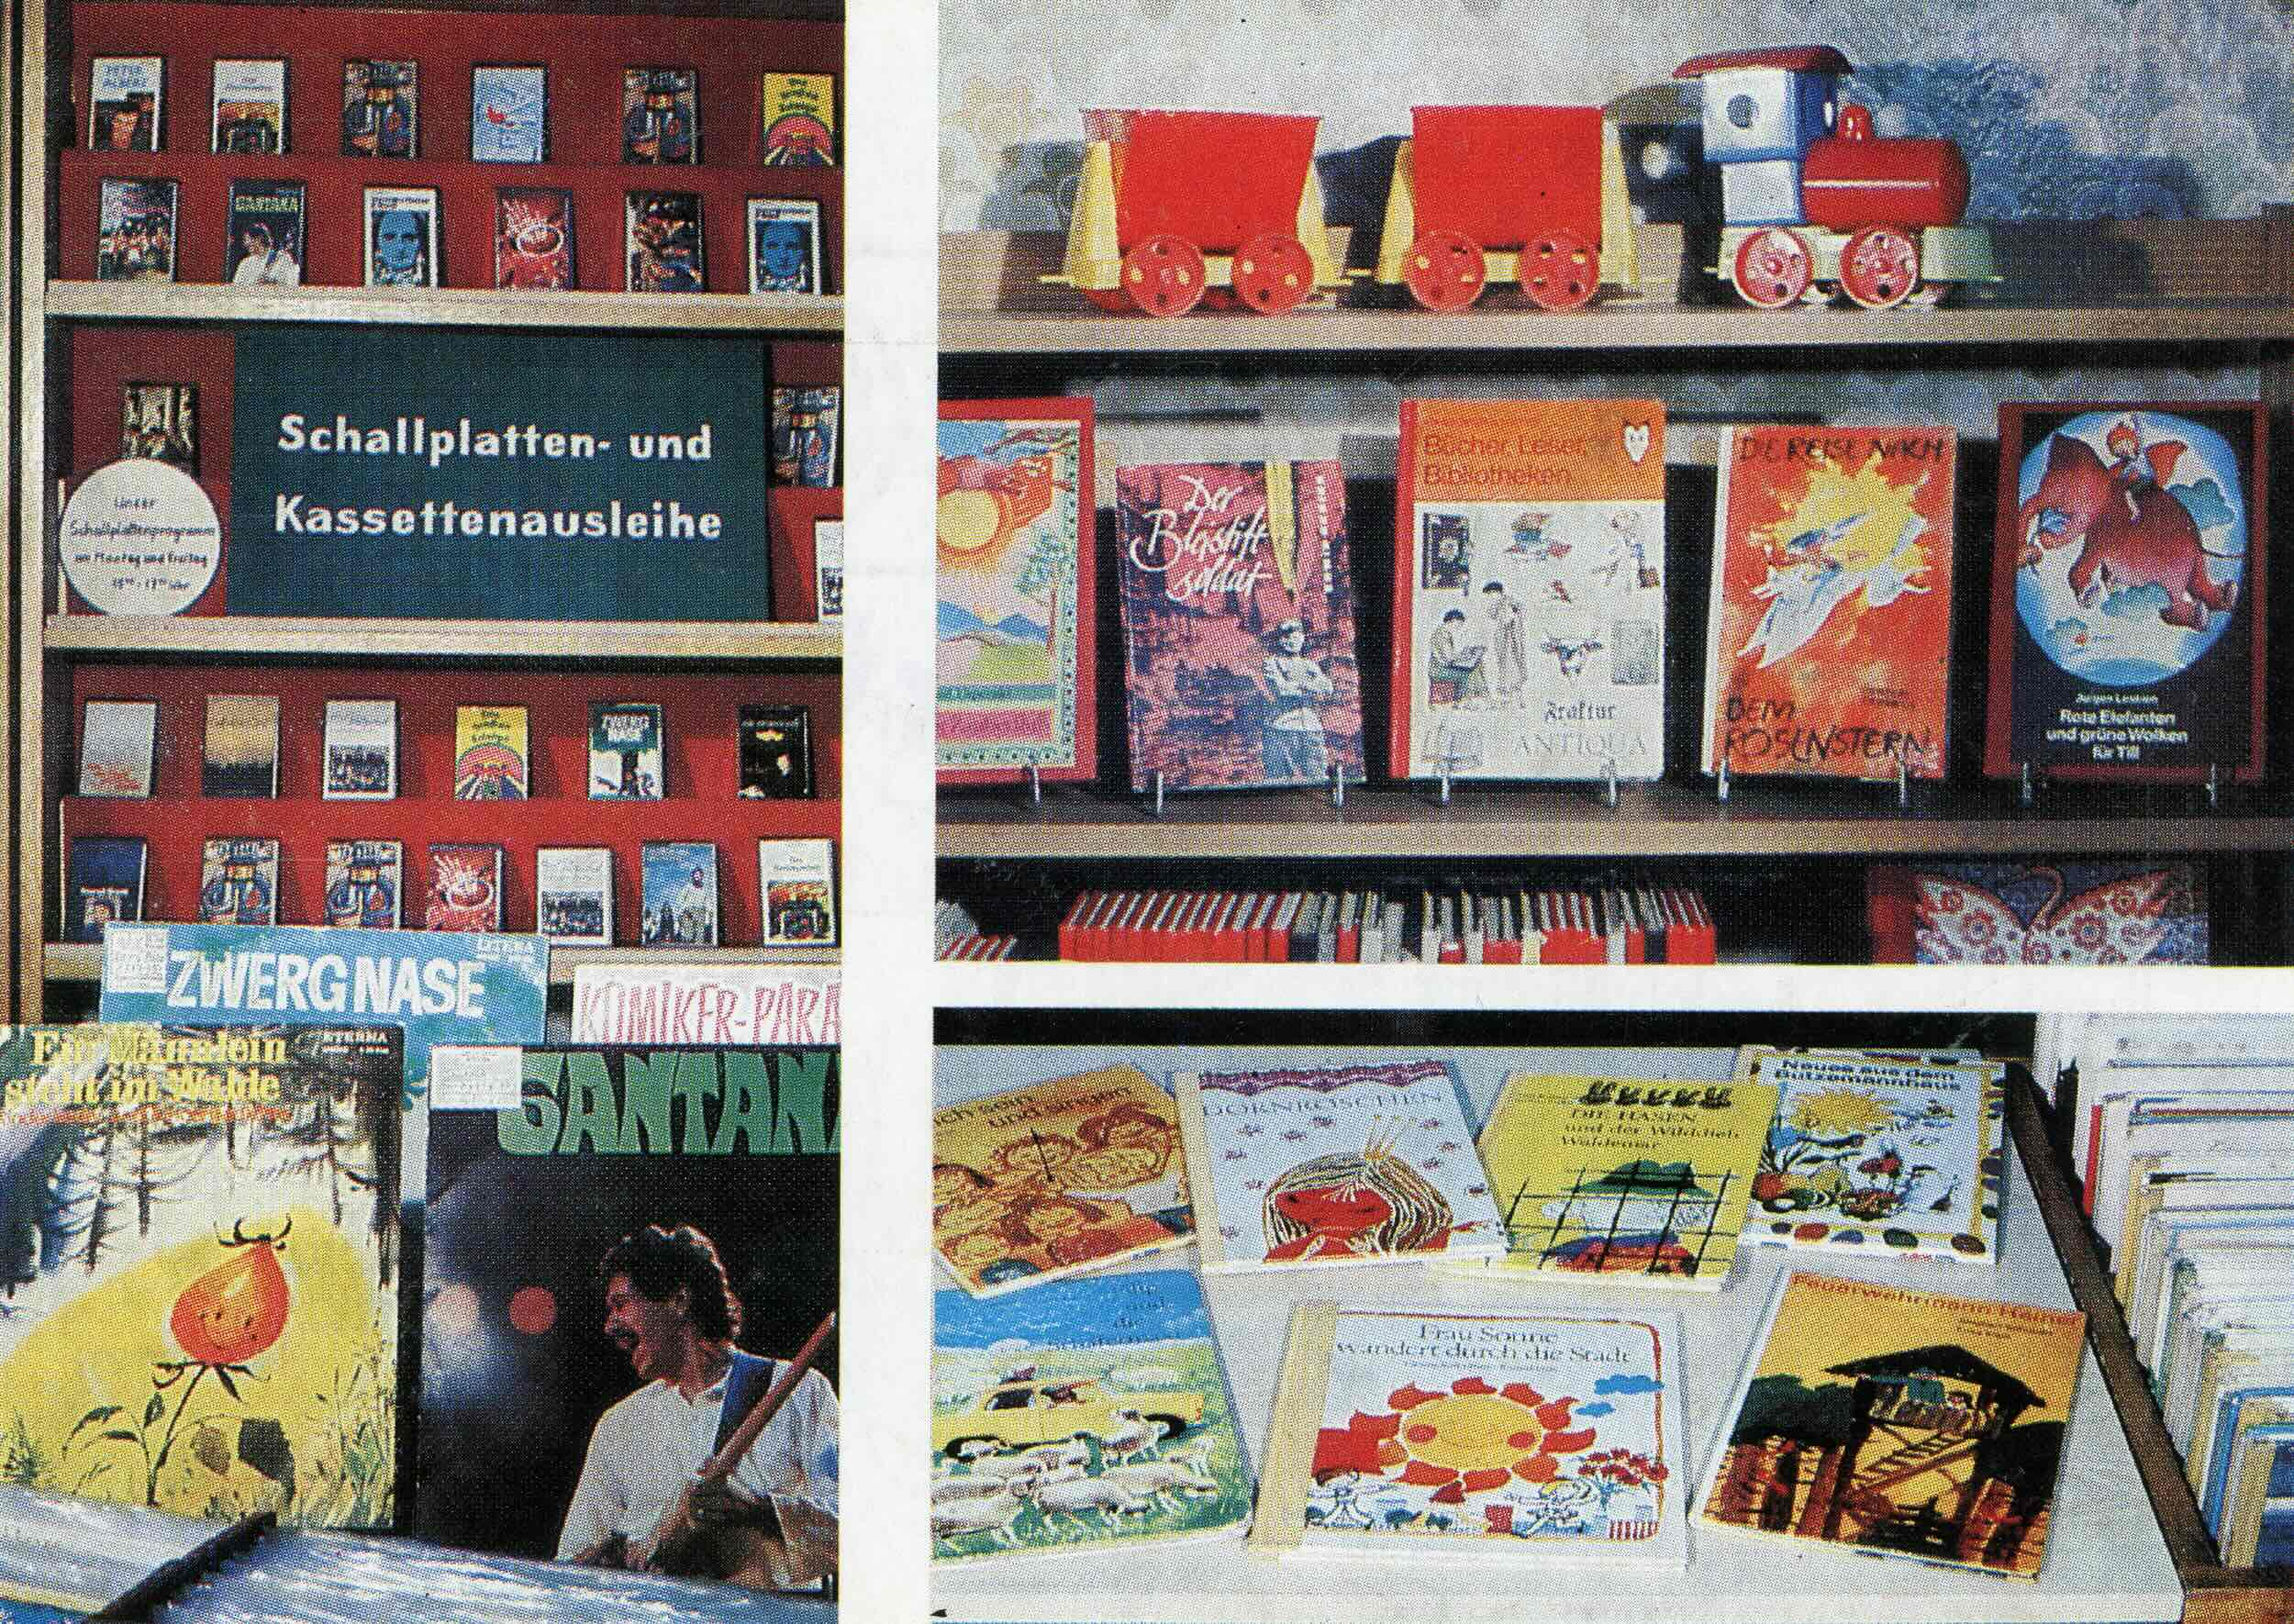
\includegraphics{img/abb1.jpg}
\caption{Ansichtskarte der Stadtbezirksbibliothek Berlin-Friedrichshain.
((204) Bp 260/78 65 3268)}
\end{figure}

Rekonstruieren lässt sich allerdings zumindest die interessante
Tatsache, dass Stadtbibliotheken in der DDR mittels eigens dafür
hergestellten Ansichtskarten Öffentlichkeitsarbeit oder besser noch
Beziehungspflege mit den bei ihnen registrierten Nutzenden betrieben.
Für die Kinderbibliothek in der Wedekindstraße waren es immerhin um die
2.000 Personen, sofern man der zeitgenössischen Presse glauben
mag.\footnote{Neues Deutschland, 25.02.1975, S.\,8}

Die Ansprache der Zielperson war entsprechend persönlich gehalten,
wenngleich vorgedruckt. Um sich Optionen offen zu halten, begann sie mit
einem \enquote{Liebe}, das von der versenden Personen je nach gelesener
Geschlechtsspezifik der Adressierten noch ergänzt werden konnte. Im
Gegensatz zu Toni Erdmann, Toni Braxton oder Toni Morrison war Tony in
diesem Fall also ein Junge, eventuell so bereits durch das \enquote{y}
markiert. Und dieser Junge wurde von seiner Bibliothek vermisst:
\enquote{Seit Du das letzte Mal bei uns warst} -- ist etwas passiert.
Nichts Spektakuläres. Bibliothekstypisch wurde einfach der Bestand
aktualisiert.

Auffällig ist an der Nachricht, dass das Medium Schallplatte gestrichen
wurde. Neu waren also nur \enquote{viele Bücher und Kassetten}. Aus der
Antizipation, dass auch für Tony die richtigen Neuerscheinungen dabei
sein dürften, erfolgte schließlich verbalisiert die Erwartung eines
ebenfalls neuerlichen Besuchs der Bibliothek. Die Botschaft folgt einem
denkbar einfachen appellativen Dreischritt des Marketings: (1) Du, in
diesem Fall als Nutzer und nicht als Kunde, bist uns wichtig. (2) Wir
haben etwas Neues im Angebot. (3) Schau es Dir an. Dazu viele Grüße,
aber leider nicht per Hand unterzeichnet, sondern nur mit dem
Kontaktstempel. Das schwächt das Ansprachesignal wiederum ab. Was genau
soll Tony mit der im Stempelbild gelieferten Telefonnummer anfangen?
Anrufen und erfragen, was es denn genau Neues gibt und ob sich der Gang
wirklich lohnt? Angesichts der überschaubaren Telefonausstattung von
Haushalten in der DDR war nicht einmal gesetzt, dass dies zum
Ortsgespräch aus dem Wohnungsflur möglich gewesen wäre. Am
Comenius-Platz hätte es einen öffentlichen Münzfernsprecher gegeben.
Aber da wäre man schon fast bei der Bibliothek und könnte sich die
zwanzig Pfennig sparen.

Die auf der Karte angegebenen Öffnungszeiten verweisen auf einen
Abgleich mit dem Schulbetrieb. Da die Kinderbibliothek in der
Wedekindstraße auch die umliegenden Schulen versorgte\footnote{Ebenda},
ist davon auszugehen, dass man vormittags auch mal in die Einrichtungen
ging. Der Mittwoch fiel aus, denn an diesem fand der Pioniernachmittag
statt und machte die Kinder in Friedrichshain mit den Zielen, Rollen und
Möglichkeiten der sozialistischen Gesellschaft vertraut. Beispielsweise
durch das Sammeln von Altpapier, was an guten Tagen durchaus mal eine
Ausgabe des \enquote{Neuen Leben} oder der \enquote{NBI} und an noch
besseren sogar eine Ausgabe der Zeitschrift \enquote{Das Magazin} in die
kleinen Hände der die Treppenhäuser durchsteigenden
Altstoffsammler*innen brachte. Diese besonderen Drucke verließen die
sorgsam verschnürten Zeitungspakete oft wie von selbst auf dem Weg zur
nächsten Sekundärrohstoffannahmestelle, von der es eine auf halbem Weg
zwischen Tonys Adresse und der Kinderbibliothek gab, und wurden
anschließend zur mehr oder weniger heimlichen Lektüre der jungen
Pioniere und / oder ihrer älteren Geschwister.

Eine Besonderheit der kulturellen Übersichtlichkeit, wie sie die DDR
kennzeichnete, war, dass sich die meisten jungen Menschen tatsächlich
sehr offen und intensiv mit dem konfrontierten, was zufällig greifbar
wurde. So besprach der Jugendjournalismus nicht nur die neuesten Pop-
und Schlagerveröffentlichungen, sondern auch neue Pressungen bei ETERNA,
dem Label für klassische Musik. Wer darüber gelesen hatte, fand dann
auch diese Tonträger in den sperrholzigen Schallplattenstellboxen
mancher Kinderbibliothek.

Auch die auf der Bildseite der Erinnerungskarte erkennbaren Titel
spiegeln den eklektischen Mix der medialen Bildungsreise junger Menschen
in der DDR. Hier treffen die hellen Stimmen des Kleinen Kinderchors des
Deutschlandsenders (\enquote{Ein Männlein steht im Walde}) auf Samba Pa
Ti (Santana). Dahinter warten in der \enquote{Komiker-Parade} Aufnahmen
von Lutz Jahoda, Lotte Werckmeister und natürlich Rolf Herricht und
Hans-Joachim Preil für alle, die \enquote{Zwerg Nase} in der
Hörspielfassung mit niemand Geringerem als dem DEFA-Star Angelica
Domröse in der Stimmrolle der Gans bereits durchgehört haben.

\begin{figure}
\centering
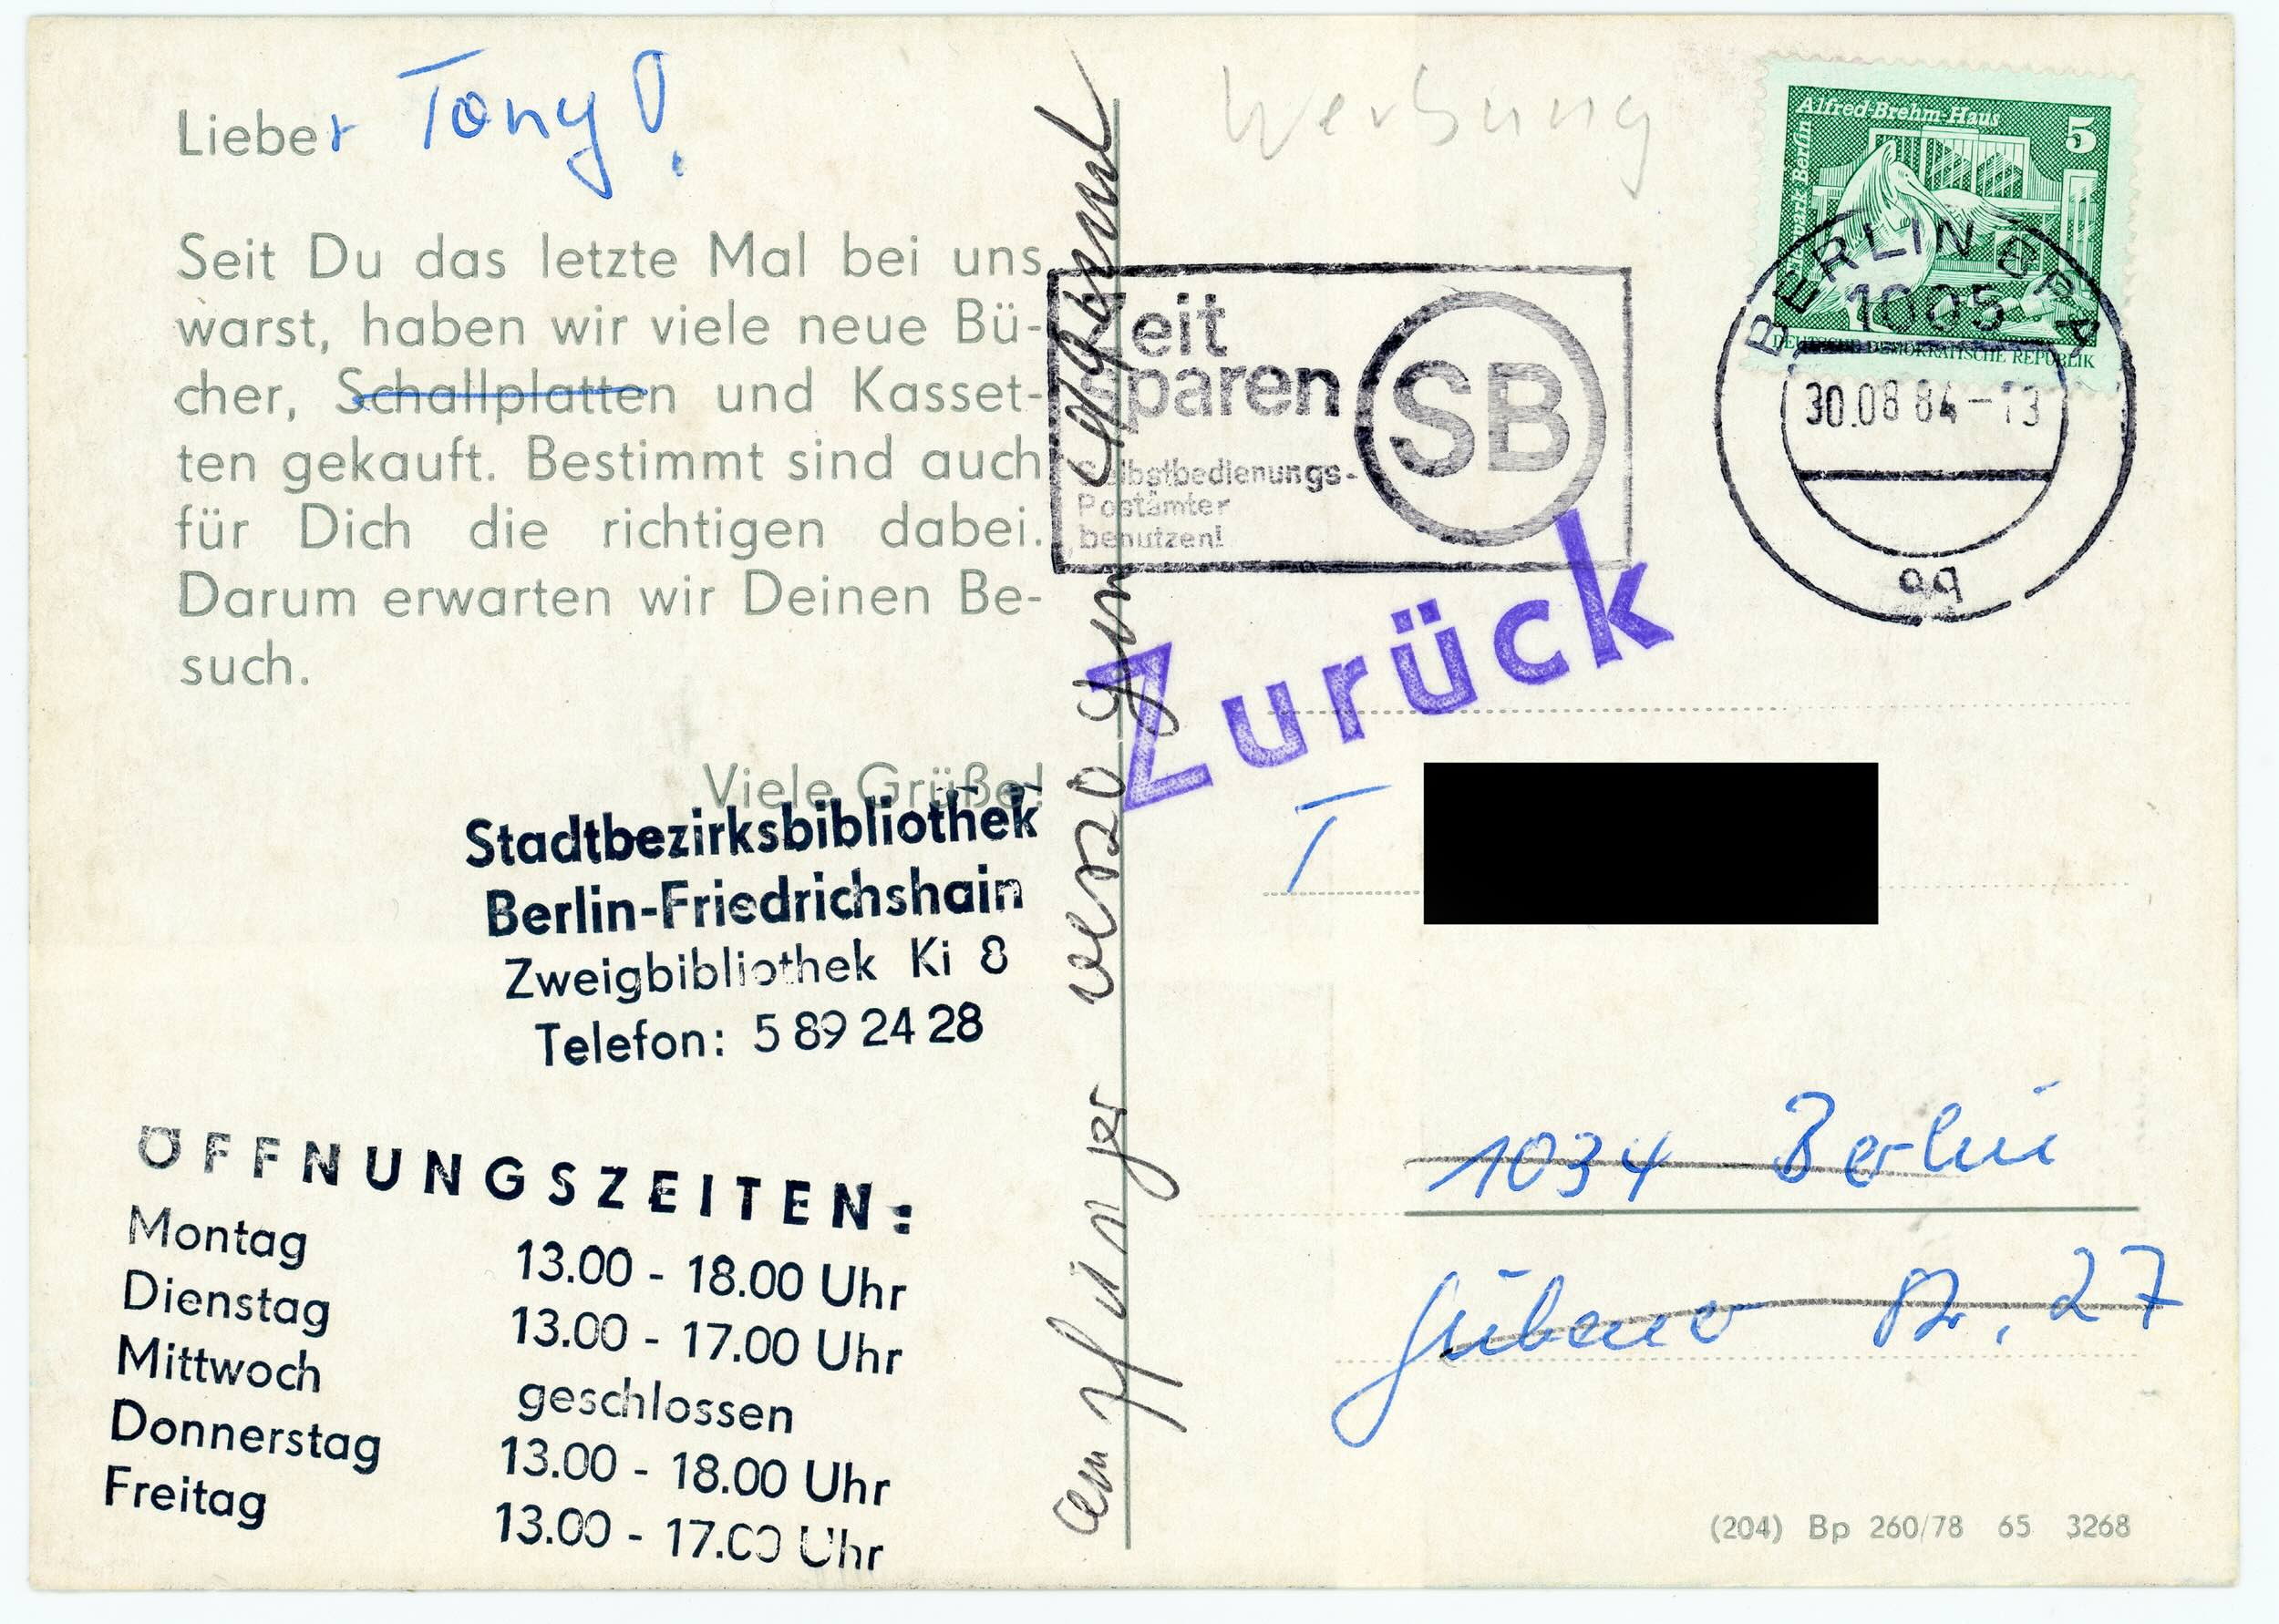
\includegraphics{img/abb2.jpg}
\caption{Ansichtskarte der Stadtbezirksbibliothek Berlin-Friedrichshain.
((204) Bp 260/78 65 3268)}
\end{figure}

Das Buchangebot bildet die Kinderbücher der DDR-Gegenwart ab: Da wären
Erwin Bekiers Geschichte des sowjetischen Frontzeichners Wladimir
Bogatkin und Herbert Friedrichs vielfach aufgelegtes Sci-Fi-Märchen
\enquote{Die Reise nach dem Rosenstern}. Zwischen beiden wiederum
leuchtet das Leitbuch aller DDR-Kinder, die die Bibliothek nicht nutzen,
sondern irgendwann auch einmal als Arbeitsort haben wollten: das von
Hansgeorg Meyer verfasste und von Gisela Wongel illustrierte
Kinderlexikon \enquote{Bücher, Leser, Bibliotheken}.
\enquote{Unterhaltsam werden junge Leser mit den Möglichkeiten der
Bibliotheksbenutzung, mit der Anfertigung einer eigenen Bücherkartei,
mit einigen früher und heute gebräuchlichen Schriften usw. bekannt
gemacht.} schrieb Helmut Casper 1977 in seiner Rezension zur ersten der
mindestens sechs Auflagen.\footnote{Helmut Casper: Unterhaltsames
  Lexikon für Bücherfreunde. In: Neues Deutschland, 19./20. Februar
  1977, S.\,14}

Wer sich jetzt wundert, warum eine Karte, die neue Bücher verspricht,
Bücher zeigt, die zum Sendezeitpunkt sieben und mehr Jahre alt waren,
kann sich anhand der Druckgenehmigungsnummer am unteren Rand der
Mitteilungsseite aufklären. Die datiert für diese Ansichtskarte auf das
Jahr 1978 und zeigt damit, dass die Karten entweder doch nicht so oft
verschickt oder in einer mehr als ein halbes Jahrzehnt füllenden
Vorratsauflage angefertigt wurden.

Mir selbst kam das Motiv bislang eher selten unter, was für die erste
Deutung spricht. Oder auch dafür, dass solche Postsendungen kaum von
jemandem aufgehoben wurden. Ich bewahre sie selbstverständlich in meiner
kleinen Ansichtskartensammlung, denn als jemand aus der Generation, die
1986 selbst in Kinderbibliotheken der DDR unterwegs war, ist der reiche
\enquote{Text} dieses Exemplars zugleich ein weitschwingendes
Zugangsportal zu meiner eigenen Mediensozialisation.

Da zu meiner kleinen Heimatstadtbibliothek keine expliziten Karten
dieser Art im schmalen Materialbestand zu meiner eigenen Kindheit
überliefert sind, kann ich als Ergänzung nur eine Außenansicht auf einen
Ort mit einer frühen Bibliotheksprägung einschieben: das Pionierhaus im
Pionierweg in Eisenhüttenstadt vom gegenüberliegenden Kindergarten aus
gesehen. Die Bibliothekszimmer lagen, wenn ich mich richtig erinnere, im
Gebäude zur Hofseite. Und ich erinnere mich vermutlich richtig, denn zur
Straßenseite lagen unter anderem die Übungszimmer der Musikschule und
die Klangkulisse, die die zur Bibliothek eilenden Kinder schon außerhalb
des Bildrandes empfing, hallt bis heute nach.

\begin{figure}
\centering
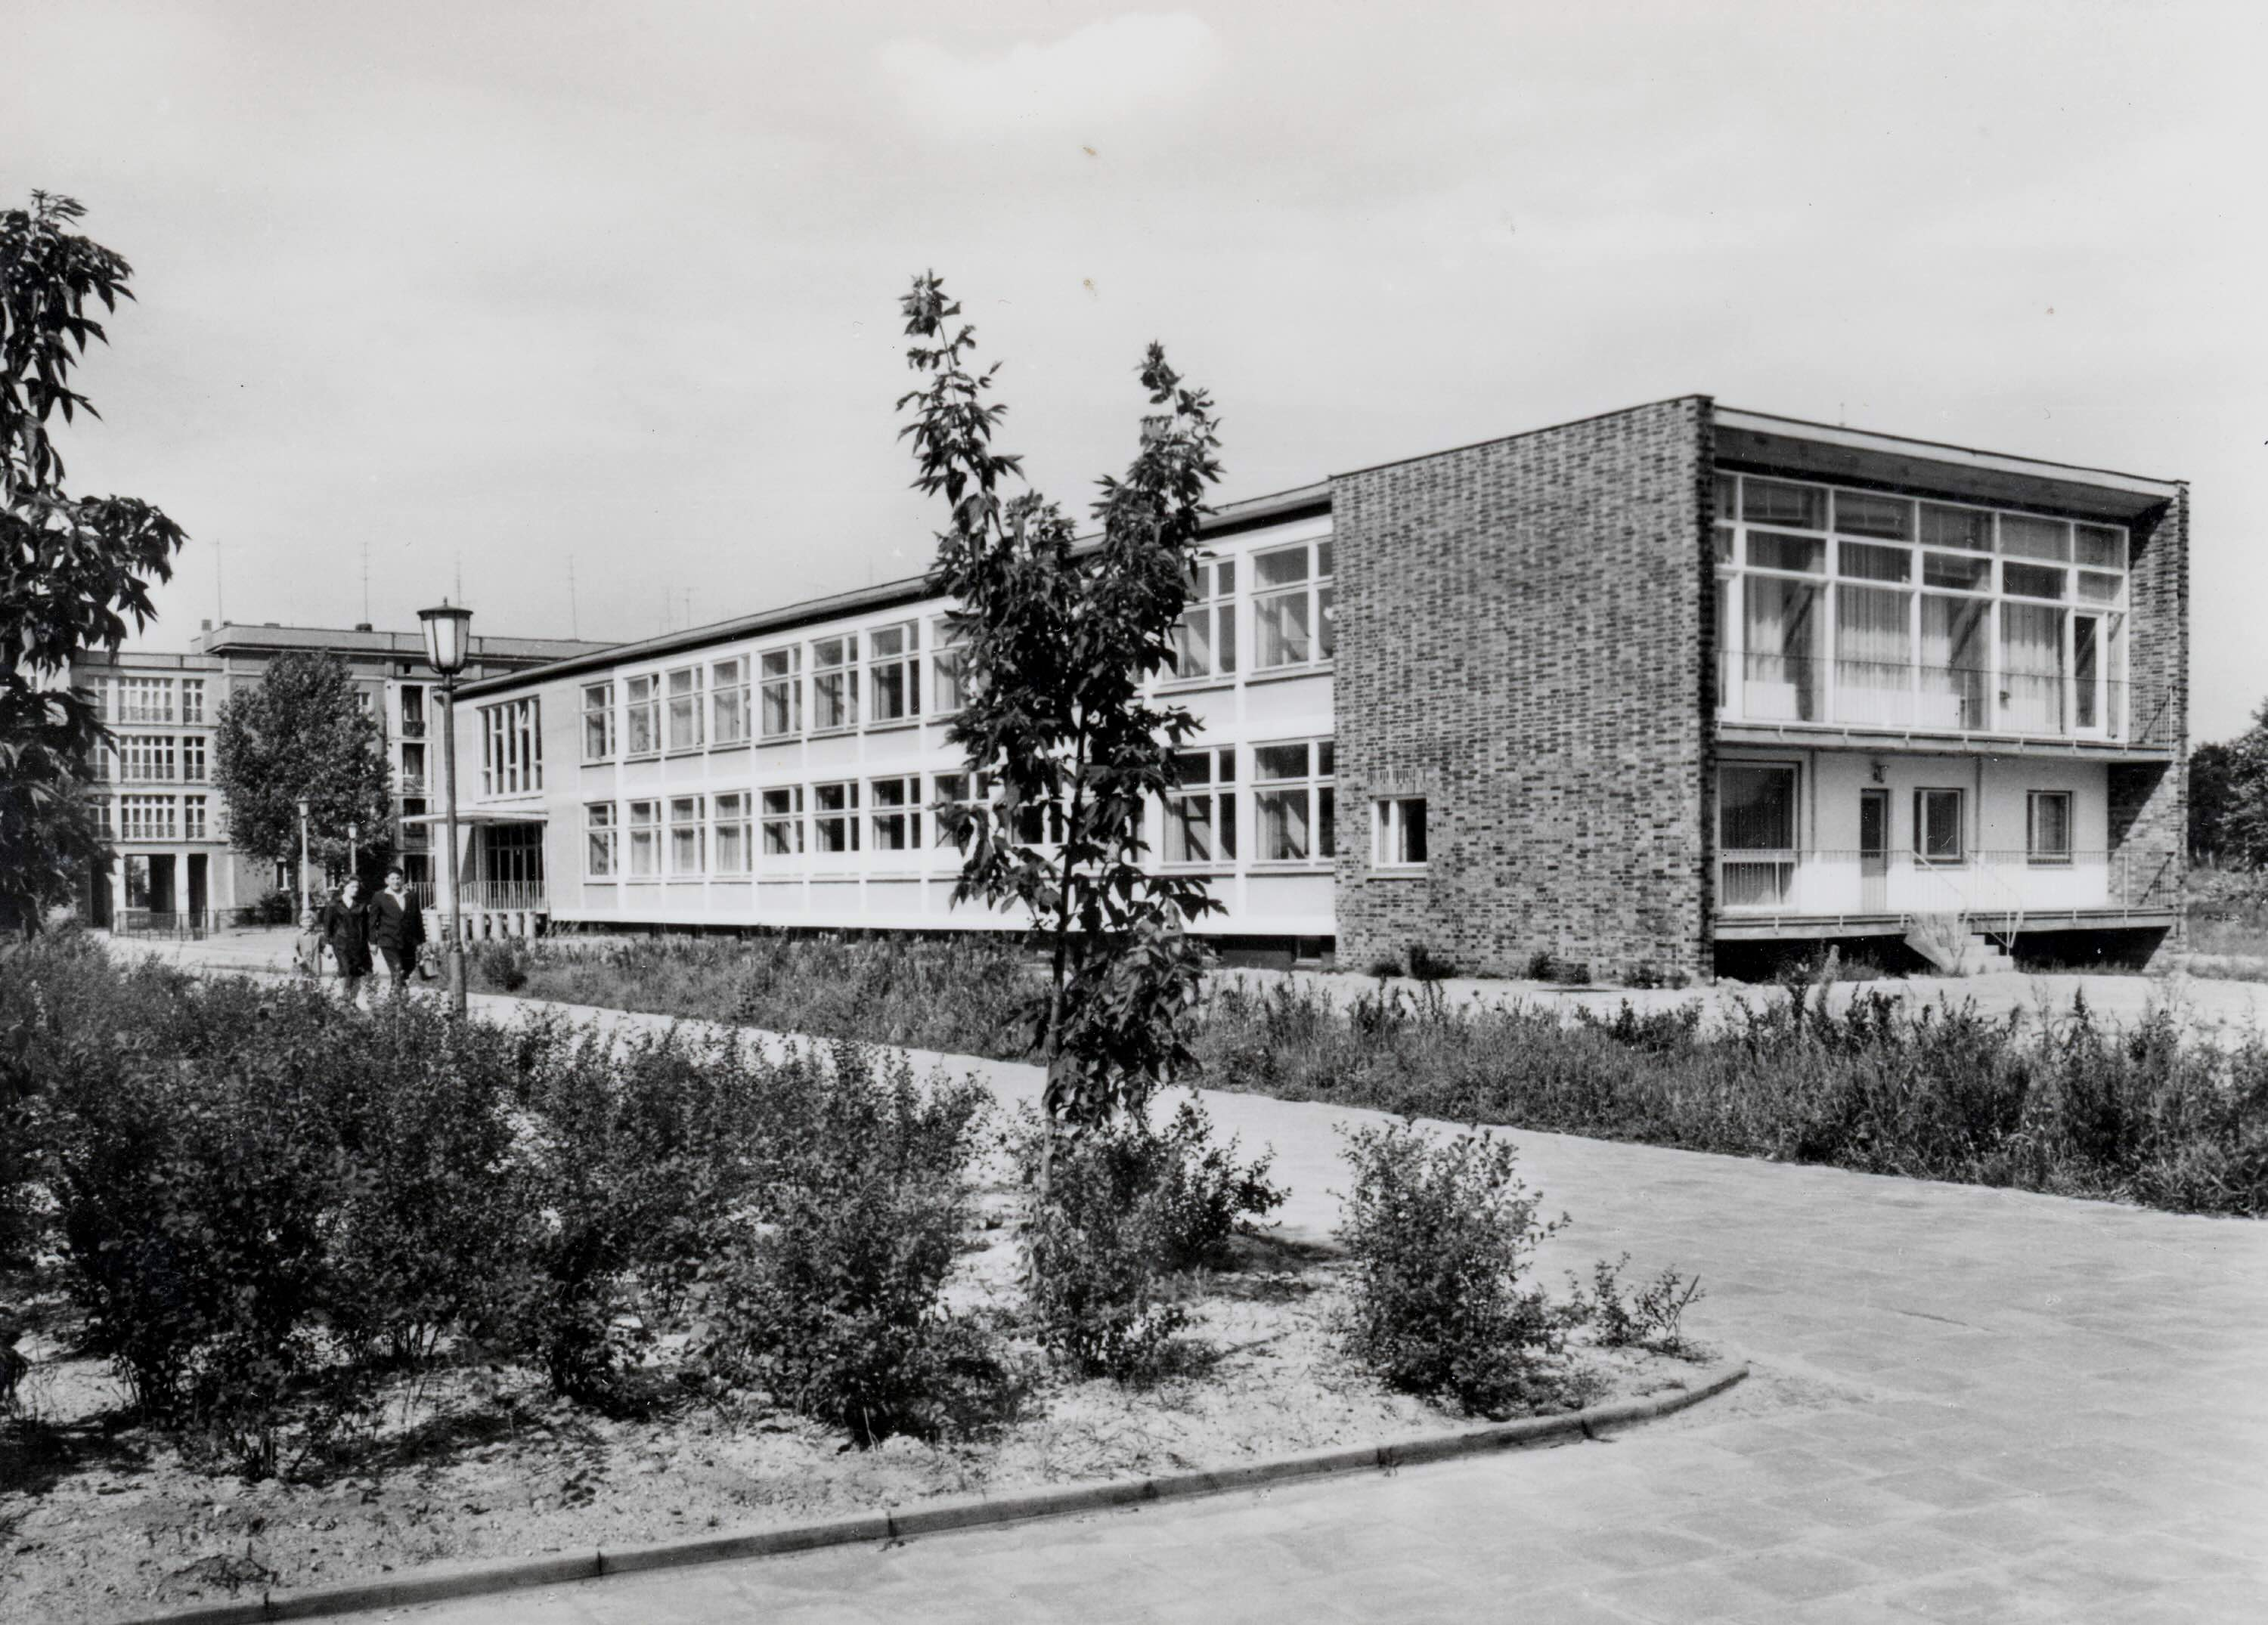
\includegraphics{img/abb3.jpg}
\caption{Ansichtskarte: Eisenhüttenstadt. Schule-Pionierhaus. Am
Pionierweg. Berlin: Graphokopie H. Sander KG, 1071 Berlin (B 8/68
Best.-Nr. B 2759). 1968}
\end{figure}

Wieso ausgerechnet das mir vorliegende Exemplar der Friedrichshainer
Bibliothekskarte überlebte, wird vermutlich für immer ein Rätsel
bleiben. Aus Tonys eigener Sammlung wird sie aller Wahrscheinlichkeit
nach nicht stammen und zwar nicht deshalb, weil ich den Berliner
Innenring-Kids der späteren Generation Ostgut nicht zutraue, sich auch
der philokartistischen Nostalgie hinzugeben. Sondern, weil diese Karte
ihren Adressaten nie erreichte. \enquote{Empfänger verzogen} zieht sich
in eiliger Zusteller*innenschrift an der Trennlinie der Karte entlang.
Und im zeittypischen immergrünen Stempellila prangt dazu ein Wort, das
zugleich das Motto meiner Blicke auf derartige Ansichtskarten sein
könnte: \enquote{Zurück}.

%autor
\begin{center}\rule{0.5\linewidth}{0.5pt}\end{center}

\textbf{Ben Kaden} ist Herausgeber der LIBREAS.Library Ideas.

\end{document}